\chapter{The growth of social groups}
\label{Ch:Groups}

The evolving complex networks have tendency to separate into connected fragments, communities ot groups of nodes. These communities are formed around certain topics, interests, and they play important role in shaping the structure and dynamics of the network. The distribution of the sizes of these communities has universal shape. To understand how the dynamics and structure of the networks affects the distribution of community sizes we combine the empirical approaches and theoretical modeling. We analyse real-world social networks, collect data about their structure and community sizes, while theoretical modeling involves developing models able to capture essential features of social networks and explain emergence of universal distribution od group sizes.

%%TODO Ovde nedostaje jedan paragraf pre ovoga koji objašnjava zašto ovo izučavamo. Nešto na sledeću temu: "Some of the evolving complex networks have tendency separate into connected fragments, communities or groups of nodes. In the case of social networks, these communities are seen as the groups of members who are grouped around certain topics or other common traits. As a social network evolves so does its segmentation into groups. The segmentation is closely related to social network structure and members' preferences. The distribution of the sizes of social groups often has an universal shape.  We combine empirical approach and theoretical modeling to study study how the shape of this distribution depends on the network structure."  Možda ovaj pasus da ide pre ove sekcije

\section{Empirical analysis of the social group growth}
%%TODO Ne "Social groups" nego "Empirical analysis of the social group growth"

Two popular online platforms, \textbf{Reddit} and \textbf{Meetup}, are organized into different groups. On Reddit \footnote{https://www.reddit.com/}, users create subreddits, where they share web content and discussion on specific topics, so their interactions are online through posts and comments. The Meetup groups \footnote{www.meetup.com} are also topic-focused, but the primary purpose of these groups is to help users in organizing offline meetings. As meetings happen face-to-face, Meetup groups are geographically localized, so we'll focus on groups created in two towns, London and New York.  

The Meetup data cover groups created from $2003$, when the Meetup site was founded, until $2018$, when we downloaded data using the Meetup API. We extracted the groups from London and New York that were active for at least two months. There were 4673 groups with 831685 members in London and $4752$ groups with 1059632 members in New York. For each group, we got information about organized meetings and users who attended them. From there, for each user, we can find the date when the user participated in a group event for the first time; it is considered the date when the user joined a group. 

The Reddit data were downloaded from the https://pushshift.io/ site. This site collects posts and comments daily; data are publicly available in JSON files for each month. The selected subreddits were created between 2006 and 2011, and we filtered those active in 2017. We removed subreddits active for less than two months. The obtained dataset has 17073 subreddits with $2 195 677$ active members. For each post, we extracted the subreddit-id, user-id and the date when the user created the post. Finally, we selected the date when each user posted on each subreddit for the first time. 

\subsection{The empirical analysis of social groups}

We have information about when the user attended the group event for each Meetup group. In contrast, we have detailed data about user activity for the subreddit, so we can extract the information when a user creates a post for the first time. Those dates are considered as the timestamp when a user joins to group. So both datasets have the same structure: $(g, u, t)$, where $t$ is the timestamp when user $u$ joined group $g$. For each time step, we can calculate the number of new members in each group $N_i(t)$, and the group size $S_{i}(t)$. The group size at time step $t$ is $S_{i}(t)=\sum^{k=t}_{k=t_{0}}N_{i}(t)$, where $t_0$ is month when group is created. The group size is increasing over time, as we do not have information if the user stopped to be active. Also, we calculate the growth rate as the logarithm of successive sizes $R = log(S_{i}(t)/S_{i}(t-1))$.

Even though Meetup and Reddit are different online platforms, we find some common properties of these systems; see Figure \ref{fig:data1}. The number of groups and the number of new users grow exponentially. Still, subreddits are larger groups than Meetups. The distribution of groups sizes follows the lognormal distribution:
\begin{equation}
P(S)=\frac{1}{S\sigma\sqrt{2\pi}}exp(-\frac{(\ln(S)-\mu)^{2}}{2\sigma^{2}})
\label{eq:log}
\end{equation}
where $S$ is the group size and $\mu$, and $\sigma$ are parameters of the distribution.

\begin{figure}[h]
	\centering
	\includegraphics[width=0.8\linewidth]{chapter4/Fig2.png}
	\caption[Properties of Meetup and Subreddit groups]{The number of groups over time, normalized sizes distribution, normalized log-rates distribution and dependence of log-rates and group sizes for Meetup groups created in London from 08-2002 until 07-2017 that were active in 2017 and subreddits created in the period from 01-2006 to the  12-2011 that were active in 2017. }
	\label{fig:data1}
\end{figure}   

The distributions for Meetup group sizes in London and New York follow a similar lognormal distribution, with parameters $\mu= -0.93$, $\sigma = 1.38$ for London and $\mu=-0.99$ and $\sigma=1.49$ for New York. The group sizes distribution of Subreddits is a broad lognormal distribution that resembles the power law; it has parameters $\mu= -5.41$ and $\sigma = 3.07$.   Still, we used the log-likelihood ratio method and showed that lognormal distribution is a better fit for these data than the power-law. The Result section is given a detailed analysis that supports these findings.   

The simplest model that generates the lognormal distribution is the multiplicative process \cite{mitzenmacher2004brief}. Gibrat used this model to explain the growth of firms. The main assumption of this model is that growth rates  $R = log\frac{S_t}{S_{t-\Delta t}}$ do not depend on the size $S$ and that they are uncorrelated. Further, this implies the lognormal distribution of the sizes, while the distribution of growth rates appears to be a normal distribution,  \cite{mondani2014fat}, \cite{fu2005growth}. Figure \ref{fig:scale} shows the distribution of the logrates that follow a lognormal distribution, contrary to the Gibrat law. Furthermore, logrates depend on the group size \ref{fig:scale}. For these reasons, the Gibrat law can not explain the growth of online social groups. Similar conclusions are shown in recent studies about cities or the growth of the internet \cite{frasco2014spatially, qian2014origin}.   

\begin{figure}[h]
	\centering
	\includegraphics[width=0.8\linewidth]{chapter4/Fig1.png}
	\caption[Universality in the Meetup and Reddit groups]{The figure shows the groups' sizes distributions and log-rates distributions. Each distribution collects groups founded in the same year and is normalized with its mean value. The group sizes are at the end of 2017 for meetups and 2011 for subreddits.}
	\label{fig:scale}
\end{figure}

The growth of online social groups has universal behavior independent of the group's size. If we aggregate the groups created in the same year $y$, and each group size normalizes with average size $<S^y>$, $s^{y}_{i}=S^{y}_{i}/<S^{y}>$ we will find that group sizes distributions for the same dataset and different years fall on the same line, Figure \ref{fig:scale}. The same characteristics are observed for the distribution of the normalized logrates \ref{fig:scale}. The growth is universal over time, and the group sizes distribution does not change from year to year.

\clearpage
\newpage
\section{Theoretical model of social group growth} %%TODO Theoretical model of social group growth

Meetup and Reddit engage members in different activities. Still, there are some underlying processes same in both systems. Each member can create new groups and join existing ones. Both systems grow in the number of groups and users, and each user can belong to an arbitrary number of groups. In the previous section, we identified the universal patterns in the growth of social groups, but the growth can not be modelled with the Gibrat law. 

The complex network models allow us to simulate the growth of these systems considering all types of members' activities. We can identify how model parameters shape growth by varying linking rules.
Regarding the user's group choice, it was shown that social connections play an important role \cite{kairam2012life, zheleva2009co}. On the other hand, users can be driven by personal interests. Diffusion between groups could also be enhanced with rich-get-richer phenomena, where users join larger groups. With a complex network model, we can easily incorporate the nonlinear growth in the number of users and groups, as it is an important parameter that shapes the structure and dynamics of the complex network \cite{mitrovic2011quantitative, dankulov2015dynamics, vranic2021growth}.

The evolution of the social groups has been studied using the co-evolution model in the reference  \cite{zheleva2009co}. This model consists of two evolving networks: the bipartite network, which stores connections between users and groups and the affiliation network of social connections. At each time step, active users create new connections in the affiliation network; i.e. they make new friends. They also join existing groups or create new ones, which updates the bipartite network. The group selection can be random with probability proportional to the group size; otherwise, the group is selected through social contacts. Using this model, authors have reproduced the power-law group size distribution found in several communities, such as Flickr or LiveJournal. The empirical analysis of Meetup and Reddit groups showed that group size distribution could be lognormal, meaning that some different mechanisms control the growth of the groups.

We propose a model that is based on the co-evolution model. The main difference between those two models is how model parameters are defined. First of all, in the co-evolution model user becomes inactive after period $t_a$, which is drawn from an exponential distribution with the rate $\lambda$, while in our model probability that the user is active is constant, and the same for each user. The second difference is how groups are chosen. While in the co-evolution model probability that the user selects a group through social linking depends on the friend's degree, we give preference to groups where a user has a larger number of social contacts. We also modified the rules for random linking so users choose a group with uniform probability.

\subsection{Groups growth model}

The representation of the model is given in Figure \ref{fig:schema}. The model consists of two networks:
\begin{itemize}
	\item bipartite network $\mathcal{B}(V_{U}, V_{G}, E_{UG})$, where $V_U$ is set of users, $V_G$ set of groups and $E_{UG}$ set of links between users and groups, where link $e(u,g)$ indicates that user $u$ is member of group $g$.
	\item social network $\mathcal{G}(V_{U},E_{UU})$ describes the social connections $e(u, v)$ between users $u$ and $v$, and  $V(U)$ is set of users same as in bipartite network. 
\end{itemize}

The bipartite and social networks evolve. New users $N_U(t)$ are added to the network at each step. It is how the set of users $V_U$ in the bipartite and social network can grow. At arrival, each new member connects to a randomly selected user in the social network $G$. This allows new members to choose a group based on social contacts \cite{kairam2012life}. The activity of old members is a stochastic process; old members are activated with probability $p_a$. The set of active users $\mathcal{A}_{U}$ has new members $N_U(t)$ and old members who decided to be active in that time step.

The active users can create a new group with probability $p_g$. By this, group node $g$ is added to the set of group nodes $V_G$ in bipartite network $B$. If an active user does not create a new group, it will join the existing one with probability $1-p_g$, see lower panel on Figure \ref{fig:schema}. When the user creates a new group or joins an existing one, the link $e(u,g)$ is made in the bipartite network $B$.

\begin{figure}[h]
	\centering
	\includegraphics[scale=0.45]{chapter4/test.png}
	\caption[Bipartite groups growth model]{The top panel shows bipartite (member-group) and social (member-member) networks. Filled nodes are active members, while thick lines are new links in this time step. In the social network, dashed lines show that members are friends but do not share the same groups. The lower panel shows the model schema, where $p_g$ is the probability that the user creates a new group, while $p_{aff}$ is the probability that group choice depends on social connections. \textbf{Example:} member $u_6$ is a new member. First, it will make a random link with node $u_4$, with probability, $p_g$ makes a new group $g_5$. With probability, $p_a$ member $u_3$ is active, while others stay inactive for this time. Member $u_3$ will, with probability $1-p_g$ choose to join one of the old groups, and with probability $p_{aff}$ linking is chosen to be social. As its friend $u_2$ is a member of group $g_1$, member $u_3$ will also join group $g_1$. When member $u_3$ joins to group $g_1$, it will make more social connections; in this case, it is member $u_1$.}
	\label{fig:schema}
\end{figure}

When joining existing groups, users may be influenced by social connections. This linking happens with probability $p_{aff}$. The second case is that the user chooses a random group with probability $1-p_{aff}$. 

Social linking depends on the properties of a bipartite and social network. The networks can be represented with matrices $B$ and $A$, so if a link between two nodes exists, they have element $1$. The neighbourhood of user $u$, $\mathcal{N}_{u}$ in a bipartite network is a set of groups in which the user is a member. Similarly, we define the neighbourhood of group $g$ as $N_g$, as a set of users who belong to the group. From there, we can define the probability $ P_{ug}$ that the user $u$ will choose group $g$. This probability is proportional to the number of social contacts that the user has in the group. 

\begin{equation}
P_{ug}=\sum_{u_{1}\in \mathcal{N}_{g}} A_{uu_{1}} 
\label{eq1}
\end{equation}

After selecting group $g$, user $u$ is introduced to new members in the group and can make new social contacts. In the simplest case, we could assume that all members belonging to a group are connected. However, previous research on this subject \cite{ smiljanic2017associative, backstrom2006group, zheleva2009co} has shown that the existing social connections of members in a social group are only a subset of all possible connections. We select $X$ random members $u_i$ from a group $g$ and make new connections in the social network $e(u, u_i)$. 

The model parameters $p_a$ and $p_g$ are important for controlling the number of users and groups. With larger parameter values $p_a$, more users become active, and the number of links in bipartite and social networks grows faster. Parameter $p_g$ controls the rate at which new groups are created. For example, if $p_g=0$, users will not create new groups. Also, if $p_g=1$, users will only create new groups, and the resulting network will consist of star-like subgraphs. In real systems, we do not expect extreme values for probabilities $p_a$ and $p_g$. First, not all members are constantly active, and we do not find a burst in the creation of the groups. From real data, we notice that there is always a higher number of users than groups in social systems. The parameter $p_{aff}$ how users choose groups, and with higher $p_{aff}$ social connections become more important. 

\subsection{Dependence of the group size distribution on model parameters}

Before applying the group growth model on Meetup and Reddit, we consider the system where at each time step, a constant number of users is added $N(t)=30$. We also fix the probability that the user is active to $p_a=0.1$, so we can, in more detail, explore the influence of parameters $p_g$ and $p_{aff}$. We plot the group size distribution after the $60$ steps of simulation. The values of $p_g$ and the $p_a$ influence the number of groups, their maximum size, and the shape of group size distribution. With probability $p_g=0.1$, users create a large number of groups, over $10^4$, while with $p_g=0.5$, they are on the order of magnitude $10^5$. 

Figure \ref{fig:n30} show the obtained group size distributions with power-law and lognormal fits. Users join randomly chosen groups for a lower parameter value $p_g=0.1$ and $p_{aff}=0$. Group size distributions are approximated with lognormal. When the affiliation parameter is larger, $p_{aff}=0.5$, the lognormal distribution becomes broader, and so on, we find the larger maximum group size. If we increase the parameter $p_g=0.5$, every second active user will create a group. At this group creation rate, the group size distribution deviates from lognormal, but it is not explained with power-law either, right column on Figure \ref{fig:n30}.

\begin{figure}[H]
	\centering
	\includegraphics[width=0.6\linewidth]{chapter4/Fig5_a.png}
	%\includegraphics[width=0.8\linewidth]{figures/model_N30.png}
	\caption[Group size distribution for different model parameters]{The distribution of sizes for different values of $p_{g}$ and $p_{aff}$ and constant $p_{a}$ and growth of the system. The combination of the values of parameters of $p_{g}$ and $p_{aff}$ determine the shape and the width of the distribution of group sizes. }
	\label{fig:n30}
\end{figure}

Finally, we compare how group size distribution depends on different rules in random linking. In our model, the probability that the user chooses a random group is uniform. In contrast, in the co-evolution model \cite{zheleva2009co}, probability depends on the group size, as in the preferential attachment model. Instead of random linking, if we incorporate preferential linking, users with probability $1-p_{aff}$ tend to choose larger groups, and group size distribution changes significantly. Similar to the co-evolution model, we find the power-law distribution. Figure \ref{fig:model_comp} shows the results from a model where we add a constant number of new users at each time step. The probabilities $p_a$ and $p_g$ are fixed, and the affiliation parameter takes values $0$, $0.5$ and $0.8$. If we consider random linking, a top panel on Figure \ref{fig:model_comp}, the distribution becomes broader with larger $p_{aff}$. On the other hand, with preferential linking, group size distribution is a power law, and the $p_{aff}$ parameter does not have a large impact on the distribution shape.    

\begin{figure}[h]
	\centering
	\includegraphics[width=0.7\linewidth]{chapter4/model_N30.png}
	\caption[Comparison between preferential and random linking in the groups' growth model.]{Groups sizes distributions for groups model, where at each time step the constant number of users arrive, $N=30$ and old users are active with probability $p_a=0.1$. Active users make new groups with probability $p_g=0.1$, while we vary affiliation parameter $p_{aff}$. With probability, $1-p_{aff}$, users choose a group randomly. The group sizes distribution (top row) is described with a lognormal distribution. The distribution has a larger width with a higher affiliation parameter, $p_{aff}$. The bottom row presents the case where with probability $1-p_{aff}$, users prefer larger groups. For all values of parameter $p_{aff}$, we find the power-law group sizes distribution.}
	\label{fig:model_comp}
\end{figure}

\newpage
\section{The growth of real social groups} %%TODO The growth of real social groups

The social systems do not grow at a constant rate. In Ref. \cite{vranic2021growth}, authors have shown that features of growth signal influence the structure of social networks. For these reasons, we use the real growth signal from Meetup groups located in London and New York and Reddit community to simulate the growth of the social groups in these systems. Figure \ref{fig:fig5} top panel shows the time series of the number of new members that join each of the three systems each month. All three systems have relatively low growth initially, which accelerates as the system becomes more popular.

\begin{figure}[h]
	\centering
	\includegraphics[width=0.7\linewidth]{chapter4/Fig3.png}
	\caption[The estimation of the model parameters for a groups growth model.]{The time series of the number of new members (top panel), the ratio between old members and total members in the system (middle panel), and the ratio between new groups and active members(bottom panel) for Meetup groups in London,  Meetup groups in New York, and subreddits. }
	\label{fig:fig5}
\end{figure}

We also use empirical data to estimate $p_{a}$, $p_{g}$ and $p_{aff}$. Probabilities that old members are active $p_a$ and that new groups are created $p_g$ can be approximated directly from the data. Activity parameter $p_{a}$ is the ratio between the number of old members active in month $t$ and the total number of members in the system at time $t$. Figure \ref{fig:fig5} middle row shows the variation of parameter $p_{a}$ during the considered time interval for each system. The values of this parameter fluctuate between $0$ and $0.2$ for London, and New York-based Meetup groups, while for Reddit, it ranges between $0$ and $0.15$.
To simplify our simulations, we assume that $p_{a}$ is constant in time and estimate its value as its median value during the $170$ months for Meetup systems and $80$ months of the Reddit system. For Meetup groups based in London and New York, $p_{a}=0.05$, while Reddit members are more active on average, and $p_{a}=0.11$ for this system.

Figure \ref{fig:fig5} bottom row shows the evolution of parameter $p_{g}$ for the three considered systems. The $p_{g}$ in month $t$ is estimated as the ratio between the groups created in month $t$ $Ng_{new}(t)$ and the total number of groups that month $Ng_{new}(t)+Ng_{old}(t)$, i.e., $p_{g}(t)=\frac{Ng_{new}(t)}{N_{new}(t)+N_{old}(t)}$. We see from Figure \ref{fig:fig5} that $p_{g}(t)$ has relatively high values at the beginning of the system's existence. In the beginning, these systems have a relatively small number of groups and often cannot meet the needs for the content of all their members. As time passes, the number of groups and content offerings within the system grows, and members no longer have a high need to create new groups. Figure \ref{fig:fig5} shows that $p_{g}$ fluctuates less after the first few months, and thus we again assume that $p_{g}$ is constant in time and set its value to median value during 170 months for Meetup and 80 months for Reddit. For all three systems, $p_{g}$ has the value of $0.003$.



The affiliation parameter $p_{aff}$ cannot estimate directly from the empirical data. For these reasons, we simulate the growth of social groups in each of the three systems with the time series of new members obtained from the real data and estimated values of parameters $p_a$ and $p_g$, while we vary the value of $p_{aff}$. For each of the three systems, we compare the distribution of group sizes obtained from simulations for different values of $p_{aff}$ with ones obtained from empirical analysis using Jensen Shannon (JS) divergence. The JS divergence \cite{jsdivergence} between two distributions $P$ and $Q$ is defined as 
\begin{equation}
JS(P, Q) = H\left(\frac{P+Q}{2}\right) - \frac{1}{2}\left(H(P)+H(Q)\right) \label{eq2}
\end{equation}
where $H(p)$ is Shannon entropy $H(p)=\sum_x p(x)log(p(x)$. The JS divergence is symmetric, and if $P$ is identical to $Q$, $JS=0$. The smaller the JS divergence value, the better the match between empirical and simulated group size distributions. Table \ref{tab:table} shows the value of JS divergence for all three systems. We see that for London-based Meetup groups; the affiliation parameter is $p_{aff}=0.5$, for New York groups $p_{aff}=0.4$, while the affiliation parameter for Reddit $p_{aff}=0.8$. Our results show that social diffusion is important in all three systems. However, Meetup members are more likely to join groups at random, while for Reddit members, their social connections are more important regarding the choice of the subreddit.  


\begin{table}[h]
	\centering
	\begin{tabular}{|c|c|c|c|}
		\hline
		$p_{aff}$ & JS cityLondon   & JS cityNY       & JS reddit2012    \\ \hline
		0.1  & 0.0161          & 0.0097          & 0.00241          \\ \hline
		0.2  & 0.0101          & 0.0053          & 0.00205          \\ \hline
		0.3  & 0.0055          & 0.0026          & 0.00159          \\ \hline
		0.4  & 0.0027          & \textbf{0.0013} & 0.00104          \\ \hline
		0.5  & \textbf{0.0016} & 0.0015          & 0.00074          \\ \hline
		0.6  & 0.0031          & 0.0035          & 0.00048          \\ \hline
		0.7  & 0.0085          & 0.0081          & 0.00039          \\ \hline
		0.8  & 0.0214          & 0.0167          & \textbf{0.00034} \\ \hline
		0.9  & 0.0499          & 0.0331          & 0.00047          \\ \hline
	\end{tabular}
	\caption[Jensen Shannon divergence between group sizes distributions from model and data.]{Jensen Shannon divergence between group sizes distributions from model
		(in the model, we vary affiliation parameter paff) and data.}
	\label{tab:table}
\end{table}

Figure \ref{fig:fig6} compares the empirical and simulation distribution of group sizes for three considered systems. We see that empirical distributions for Meetup groups based in London and New York are perfectly reproduced by the model and chosen values of parameters. In the case of Reddit, the distribution is very broad, and the model well reproduces the tail of the distribution.
The bottom row of Figure \ref{fig:fig6} shows the distribution of logarithmic values of growth rates of groups obtained from empirical and simulated data. We see that the tails of empirical distributions for all three systems are well emulated by the ones obtained from the model. However, there are deviations which are the most likely consequence of using median values of parameters $p_{a}$, $p_{g}$, and $p_{aff}$.

\begin{figure}[H]
	\centering
	\includegraphics[width=0.8\linewidth]{chapter4/Fig4.png}
	\caption[The comparison between empirical and simulated data.]{The comparison between empirical and simulation distribution for group sizes (top panel) and logrates (bottom panel).}
	\label{fig:fig6}
\end{figure}


\subsection{Distributions fit}

We compute the log-likelihood ratio $R$ and $p$-value between different distributions and lognormal fit \cite{clauset2009power} to determine the best fit for the group size distributions. Distribution with a higher likelihood is a better fit. The log-likelihood ratio R has a positive or negative value, indicating which distribution represents a better fit. To choose between two distributions, we need to calculate the p-value to be sure that R is sufficiently positive or negative and that it is not the result of chance fluctuation from the result close to zero. If the p-value is small, $p<0.1$, it is unlikely that the sign of R is the chance of fluctuations, and it is an accurate indicator of which model fits better.

Table \ref{tab:fit-data} summarizes the findings for empirical data on group size distributions from Meetup groups in London and New York, and Reddit. Using the maximum likelihood method, we obtain the parameters of the distributions \cite{power-law}. The results indicate that lognormal distribution best fits all three systems. Figure \ref{fig:fitdata} shows the distributions of empirical data and lognormal fit on data. For Meetup data, we present fit on stretched exponential distribution, which fits a large portion of data well. For subreddits, distribution is broad and potentially resembles power-law. Still, the lognormal distribution is a more suitable fit.

\begin{table}[h]
	\centering
	\caption[The likelihood ratio R and p-value for fitting empirical data]{The likelihood ratio R and p-value between different candidates and \textbf{lognormal} distribution for fitting the distribution of \textbf{groups sizes} of Meetup groups in London, New York and in Reddit. According to these statistics, the lognormal distribution represents the best fit for all communities. \\ }
	\begin{tabular}{|c||cc||cc||cc|}
		\hline
		\multirow{2}{*}{\begin{tabular}[c]{@{}c@{}}distribution \end{tabular}} & \multicolumn{2}{c||}{\begin{tabular}[c]{@{}c@{}}Meetup\\ city London\end{tabular}} & \multicolumn{2}{c||}{\begin{tabular}[c]{@{}c@{}}Meetup\\ city NY\end{tabular}} & \multicolumn{2}{c|}{Reddit}                    \\ \cline{2-7} 
		& \multicolumn{1}{c|}{R}                             & p                            & \multicolumn{1}{c|}{R}                           & p                          & \multicolumn{1}{c|}{R}         & p             \\ \hline \hline \hline
		exponential                                                                            & \multicolumn{1}{c|}{-8.64e2
			%-864.86
		}                       & 8.11e-32                     & \multicolumn{1}{c|}{-8.22e2}                     & 6.63e-26                   & \multicolumn{1}{c|}{-3.85e4} & 1.54e-100     \\ \hline
		\begin{tabular}[c]{@{}c@{}}stretched \\ exponential\end{tabular}                       & \multicolumn{1}{c|}{-3.01e2}                       & 1.00e-30                      & \multicolumn{1}{c|}{-1.47e2}                     & 7.78e-8                    & \multicolumn{1}{c|}{-7.97e1}    & 5.94e-30      \\ \hline
		power law                                                                              & \multicolumn{1}{c|}{-4.88e3}                      & 0.00                         & \multicolumn{1}{c|}{-4.57e3}                    & 0.00                       & \multicolumn{1}{c|}{-9.39e2}   & 4.48e-149 \\ \hline
		\begin{tabular}[c]{@{}c@{}}truncated \\ power law\end{tabular}                         & \multicolumn{1}{c|}{-2.39e3}                      & 0.00                         & \multicolumn{1}{c|}{-2.09e3}                    & 0.00                       & \multicolumn{1}{c|}{-5.51e2}   & 2.42e-56      \\ \hline
	\end{tabular}
	\label{tab:fit-data}
\end{table}

\begin{figure}[ht]
	\centering
	\includegraphics[width=0.8\linewidth]{chapter4/FigA1_data.png}
	\caption[The fitting of empirical group size distributions.]{The comparison between lognormal and stretched exponential fit to London and NY data,  and between lognormal and power law for Subreddits. The parameters for lognormal fits are 1) for city London $\mu=-0.93$ and $\sigma = 1.38$, 2) for city NY $\mu=-0.99$ and $\sigma = 1.49$, 3) for Subreddits $\mu=-5.41$ and $\sigma = 3.07$.  }
	\label{fig:fitdata}
\end{figure}

We use the same methods to estimate the fit for simulated group size distributions on Meetup groups in London, New York, and Subreddits. Table \ref{tab:fit_model} shows the results of the log-likelihood ratio R and $p$-value between different distributions. We conclude that lognormal distribution is most suitable for simulated group size distributions. We confirm our observations by plotting lognormal and stretched exponential fit on data, Figure \ref{fig:fit_model}.  
% Please add the following required packages to your document preamble:
% \usepackage{multirow}
\begin{table}[!ht]
	\centering
	\caption[The likelihood ratio R and p-value for fitting simulated data]{The likelihood ratio R and p-value between different candidates and \textbf{lognormal}
		distribution for fitting the distribution of \textbf{simulated group sizes} of Meetup groups in London, New York and Reddit. According to these statistics, the lognormal distribution
		represents the best fit for all communities.}
	\begin{tabular}{|c||cc||cc||cc|}
		\hline
		\multirow{2}{*}{\begin{tabular}[c]{@{}c@{}}distribution \end{tabular}} & \multicolumn{2}{c||}{\begin{tabular}[c]{@{}c@{}}Meetup\\ city London\end{tabular}} & \multicolumn{2}{c||}{\begin{tabular}[c]{@{}c@{}}Meetup\\ city NY\end{tabular}} & \multicolumn{2}{c|}{Reddit}                \\ \cline{2-7} 
		& \multicolumn{1}{c|}{R}                              & p                           & \multicolumn{1}{c|}{R}                            & p                         & \multicolumn{1}{c|}{R}         & p         \\ \hline \hline \hline
		exponential                                                                            & \multicolumn{1}{c|}{-6.27e4}                      & 0.00                        & \multicolumn{1}{c|}{-5.11e4}                    & 0.00                      & \multicolumn{1}{c|}{-1.26e5} & 7.31e-125 \\ \hline
		\begin{tabular}[c]{@{}c@{}}stretched\\ exponential\end{tabular}                        & \multicolumn{1}{c|}{-1.01e4}                      & 1.96e-287                    & \multicolumn{1}{c|}{-6.69e3}                     & 1.46e-93                  & \multicolumn{1}{c|}{-1.39e4} & 0.00      \\ \hline
		power law                                                                              & \multicolumn{1}{c|}{-2.29e5}                     & 0.00                        & \multicolumn{1}{c|}{-3.73e5}                   & 0.00                      & \multicolumn{1}{c|}{-4.38e4} & 0.00      \\ \hline
		\begin{tabular}[c]{@{}c@{}}truncated\\ power law\end{tabular}                          & \multicolumn{1}{c|}{-9.28e4}                      & 0.00                        & \multicolumn{1}{c|}{-1.55e5}                   & 0.00                      & \multicolumn{1}{c|}{-9.12e4} & 0.00      \\ \hline
	\end{tabular}
	\label{tab:fit_model}
\end{table}
\clearpage
\newpage
%\clearpage
\begin{figure}[H]
	\centering
	\includegraphics[width=0.8\linewidth]{chapter4/FigA2-model.png}
	\caption[The fitting of simulated group size distributions.]{The comparison between lognormal and stretched exponential fit to simulated group size distributions. The parameters for lognormal fits are 1) for city London $\mu=-0.97$ and $\sigma = 1.43$, 2) for city NY $\mu=-0.84$ and $\sigma = 1.38$, 3) for Subreddits $\mu=-1.63$ and $\sigma = 1.53$. }
	\label{fig:fit_model}
\end{figure}


\subsection{Users partition in bipartite network - degree distribution}

So far, the group growth model has focused on the degree distribution of groups and under what rules the universalities in the system reflected in the lognormal distribution of group sizes emerge. The model parameter $p_a$ controls the users' activity level; otherwise, it shapes the degree distribution of users in the bipartite network. As this probability is constant and uniform among all users, we do not expect rich properties of users' degree distribution. The expected distribution is exponential for growing random graph \cite{barabasi1999mean}, and the groups' growth model produces the same property. In Figure \ref{fig:users_degree}, blue dots show degree distributions of modelled Meetup and Reddit systems. This distribution is very well fitted with exponential form.
Furthermore, in empirical data, these distributions are long-tailed, green dots in Figure \ref{fig:users_degree}, so the model can not reproduce the degree distribution of the users. In real systems, the probability that the user is active does not have to be uniform and constant. The previous work proposed that each user has a specific lifetime \cite{leskovec2008microscopic}, but different linking rules could play an important role in shaping users' degree distribution. For example, $p_a$ could be preferential toward high-degree users or even be time-dependent.

\begin{figure}[h]
	\centering
	\includegraphics[width=1\linewidth]{chapter4/users_degree_expfit.pdf}
	\caption[Users degree distribution]{Users degree distribution}
	\label{fig:users_degree}
\end{figure}

\newpage
\section{Conclusions}

We apply complex network theory and statistical physics methods to describe the evolution of online social groups, Meetups in London and NewYork and Reddits. Instead of studying user interaction networks in a single group, which is a common approach, we are interested in quantifying how users interact with the system of multiple groups and determining which processes drive the growth of groups. Similar systems have been analyzed before. For example, it was found that the distribution of the cities or firms follows the lognormal and stays stable, showing universal behaviour. Contrary, the previous work on online social groups indicated that group size distributions of LiveJournal and Youtube follow power-law \cite{zheleva2009co}. On the other hand, for Meetup and Reddit, we find the emergence of lognormal distribution of group sizes, and the distribution of Reddit is much broader. Furthermore, these systems grow exponentially in the number of groups and new users. 

Meetup and Reddit may be platforms with different purposes, but on the lower level, both systems could be described with the same processes users perform: they can join existing groups or create new ones. Also, in these systems, new users constantly arrive. As we find the lognormal distribution in group sizes, our first attempt was to describe this system with the Gibrat model. It is a proportional growth size model, where group size distribution converges to the lognormal distribution while the log rates take the normal distribution. The second condition still needs to be met, so we need to use a more intricate method.

To explore the growth of these systems in more detail, we used a model where the social system is presented with evolving bipartite and social networks \cite{zheleva2009co}. The bipartite network has partitions of users and groups, and a link exists if a user is a group member. The social network describes the social connections between members. At each time step, new users arrive in the system, following the time series of new users, and with probability, $p_a$ old members decide to be also active. The active users can create a new group with probability $p_g$; otherwise, they will join existing groups. Their decision to select a group based on social connection is determined with probability $p_{aff}$; otherwise, the choice is random. %%TODO proslo vreme

We estimated model parameters $p_a$, $p_g$ and $p_{aff}$ from empirical data. We saw that model approximates well the empirical distributions. For Meetup groups in London and New York, the $p_{aff}$ parameter is smaller, while for Reddit, $p_{aff}$ is higher, resulting in broader group size distribution. It also means that for Reddit members, social connections are more important for the choice of groups. %%TODO proslo vreme

With results in this chapter, we contribute to the knowledge of the growth and segmentation of the socio-economic systems. Our work was motivated by the Co-evolution model \cite{zheleva2009co}. The authors explore the social groups in which group size distribution scales as power-law. We identified different universality class, the system where group size distribution follows log normal. Further, we marked off a set of linking rules which led to lognormal group size distribution and compared these two cases. By this, we expanded the classes of social systems that can be modelled.  









